\documentclass[12pt,a4paper]{article}
\usepackage[utf8]{inputenc}
\usepackage[spanish]{babel}
\usepackage{amsmath}
\usepackage{amsfonts}
\usepackage{amssymb}
\usepackage{geometry}
\usepackage{listings}
\usepackage{xcolor}
\usepackage{graphicx}
\usepackage{float}
\usepackage{booktabs}
\geometry{margin=2.5cm}

% Configuración de listings para código R
\lstset{
    basicstyle=\ttfamily\small,
    breaklines=true,
    breakatwhitespace=true,
    frame=single,
    language=R,
    showstringspaces=false,
    columns=flexible
}

\title{Estadística y Diseño de Experimentos\\
Ejercicios 6}
\date{27 de Noviembre, 2025}
\author{}

\begin{document}

\maketitle

\noindent\textbf{Nombre del alumnx:} \underline{\hspace{0.5cm}Martínez Buenrostro Jorge Rafael\hspace{0.5cm}}

\vspace{1cm}

En una empresa lechera se tienen varios silos para almacenar leche (cisternas de 60,000L). Un aspecto crítico para que se conserve la leche es la temperatura de almacenamiento. Se sospecha que en algunos silos hay problemas, por ello, durante cinco días se decide registrar la temperatura a cierta hora crítica. La temperatura de un día a otro es una fuente de variabilidad que podría impactar la variabilidad total.

% Please add the following required packages to your document preamble:
% \usepackage{booktabs}
\begin{table}[H]
  \centering
\begin{tabular}{cc|ccccc}
     &                        & \multicolumn{5}{c}{DIA}                                           \\
     &                        & Lunes & Martes & Miércoles & Jueves & \multicolumn{1}{l}{Viernes} \\ \hline
     & A                      & 4.3   & 4.0    & 4.3       & 3.8    & 4.4                         \\
     & B                      & 4.4   & 4.3    & 3.4       & 4.0    & 3.8                         \\
SILO & \multicolumn{1}{l|}{C} & 3.3   & 3.8    & 3.6       & 3.4    & 3.8                         \\
     & \multicolumn{1}{l|}{D} & 6.6   & 6.0    & 6.2       & 5.5    & 5.6                         \\
     & \multicolumn{1}{l|}{E} & 3.4   & 4.4    & 3.6       & 3.8    & 4.0                         \\ \hline
\end{tabular}
\end{table}

\begin{enumerate}
  \item Grafique los diagramas de caja y escriba sus primeras impresiones. ¿Percibe diferencias en temperaturas?
  \begin{figure}[H]
    \centering
    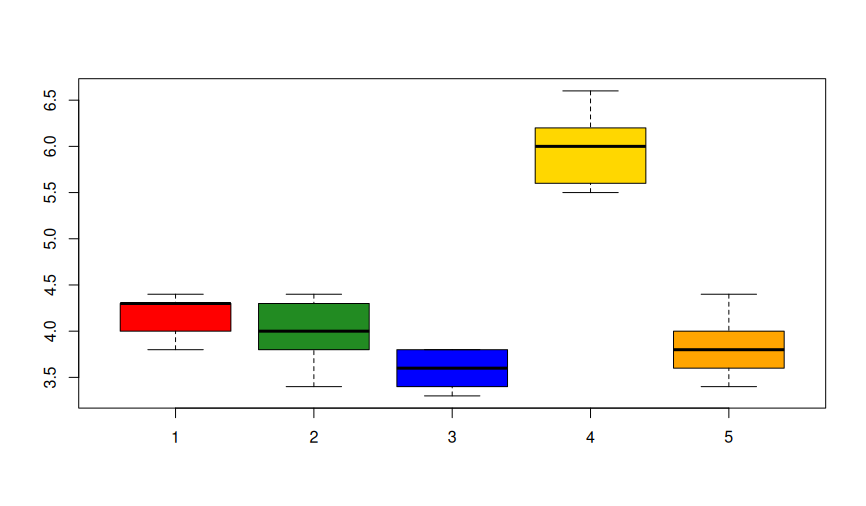
\includegraphics[width=0.6\textwidth]{img/diagramaCajas.png}
  \end{figure}

  Sí hay diferencias significativas en las temperaturas entre silos. El Silo 4 requiere atención urgente por sus temperaturas elevadas, que podrían comprometer la calidad de la leche. Los silos 1, 2, 3 y 5 parecen funcionar dentro de rangos aceptables, siendo el Silo 3 el que mejor desempeño muestra.

  \item Identifique el factor de tratamiento y el factor de bloque. Calcule las medidas importantes:
  \begin{itemize}
    \item Número de tratamientos, m: 5
    \item Número de bloques, b: 5
    \item Número de datos en cada tratamiento i: 5
    \item Número total de datos, N: 25
    \item Valores de cada media muestral \( \overline{X}_i  \): mA=4.16, mB=3.98, mC=3.58, mD=5.98, mE=3.84
  \end{itemize}

  \begin{lstlisting}[caption={Código para obtener todas las medidas importantes}]
    m <- length(unique(DatosSilos$SILO)) 
    b <- length(unique(DatosSilos$DIA))  
    n_i <- b 
    N <- nrow(DatosSilos)  

    cat("Numero de tratamientos (silos), m =", m, "\n")
    cat("Numero de bloques (dias), b =", b, "\n")
    cat("Numero de datos en cada tratamiento, n_i =", n_i, "\n")
    cat("Numero total de datos, N =", N, "\n\n")

    mA <- mean(Silo_A); mB <- mean(Silo_B); mC <- mean(Silo_C)
    mD <- mean(Silo_D); mE <- mean(Silo_E)

    vA <- var(Silo_A); vB <- var(Silo_B); vC <- var(Silo_C)
    vD <- var(Silo_D); vE <- var(Silo_E)
    cat("Medias muestrales",mA,mB,mC,mD,mE)
  \end{lstlisting}


  \item \textbf{ANOVA} Complete con ayuda de \textbf{R} la siguiente tabla del ANOVA. Recuerde que para este caso.
  \[
    F_{TRAT} = \frac{CM_{TRAT}}{CM_{ERROR}} 
  \]
  \[
    F_{BLOQ} = \frac{CM_{BLOQ}}{CM_{ERROR}}
  \]
  % Please add the following required packages to your document preamble:
  % \usepackage{booktabs}
  \begin{table}[H]
      \centering
      \begin{tabular}{@{}lllll@{}}
      \toprule
      Variabilidad & Suma de Cuadrados & Cuadrados Medios & Estadístico $F_0$ & p-valor \\ \midrule
      Tratamientos & $SC_{TRAT}=18.370$ & $CM_{TRAT}=4.593$ & $F_{TRAT}=36.276$ & 7.77e-08\\
      Bloque & $SC_{BLOQ}=0.482$ & $CM_{BLOQ}=0.121$ & $F_{BLOQ}=0.953$ & 0.46\\
      ERROR & $SC_{ERROR}=2.026$ & $CM_{ERROR}=0.127$ & & \\ \bottomrule
      \end{tabular}
  \end{table}

  \item Usando un nivel de significancia \(\alpha=0.01\), decida si se rechaza o no la hipótesis nula en el ANOVA. \textbf{Dé una interpretación}. 
  

  \item Si se rechaza la hipótesis nula en el inciso anterior, haga las múltiples comparaciones para las medias mediante el método LSD. Utilice para este punto, \(\alpha=0.05\). \textbf{Dé una interpretación}
  


  \item Escriba sus \textbf{conclusiones} para este problema.

  Estadístico \textit{l} para las comparaciones múltiples con método LSD:
  \[
    \frac{|\overline{X}_i - \overline{X}_j|}{\sqrt{\frac{2*CM_{ERROR}}{b}}}
  \]

\end{enumerate}

\newpage
\section*{Código en R}

\begin{lstlisting}

\end{lstlisting}

\end{document}